\documentclass[tikz=true]{standalone}
\usepackage[compat=1.1.0]{tikz-feynman}
\usepackage{tikz, standalone}
\usetikzlibrary{shapes.geometric, arrows, shapes.misc}
\usepackage{euler, amssymb, amsmath}
\usepackage{fontspec}
\setmainfont{MinionPro}

\begin{document}

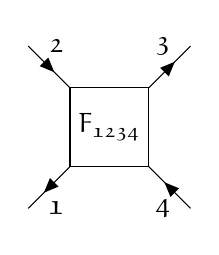
\begin{tikzpicture}[baseline=(current bounding box.center)]
    \begin{feynman}[small] % Full vertex
        \vertex (i1);
        \vertex [above right=0.75cm of i1] (a);
        \vertex [      right=of a ] (b);
        \vertex [      above=of b ] (c);
        \vertex [      left =of c ] (d);
        \vertex [      below=of d ] (a);
        \vertex [below right=0.75cm of b ] (i4);
        \vertex [above right=0.75cm of c ] (i3);
        \vertex [above  left=0.75cm of d ] (i2);
        
        \vertex [right=0.4em of i1] {$\mathfrak 1$};
        \vertex [right=0.4em of i2] {$\mathfrak 2$};
        \vertex [left=0.4em of i3] {$\mathfrak 3$};
        \vertex [left=0.4em of i4] {$\mathfrak 4$};
        
        \node (content) at ($(a)!0.5!(c)$) {$F_{\mathfrak{1234}}$};
        
        \diagram* {
            (a) -- [plain] (b) -- [plain] (c) -- [plain] (d) -- [plain] (a),
            (a) -- [fermion] (i1),
            (i4) -- [fermion] (b),
            (c) -- [fermion] (i3),
            (i2) -- [fermion] (d),
        };
    \end{feynman}
\end{tikzpicture}
\begin{tikzpicture}[baseline=(current bounding box.center)]
    \begin{feynman}
        \vertex {$=$};
    \end{feynman}
\end{tikzpicture}
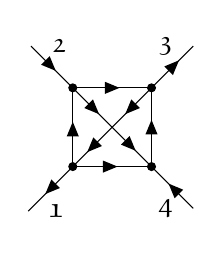
\begin{tikzpicture}[baseline=(current bounding box.center)]
    \begin{feynman}[small]
        \vertex (i1);
        \vertex [dot, above right=0.75cm of i1] (a) {};
        \vertex [dot,  right=of a] (b) {};
        \vertex [dot,  above=of b] (c) {};
        \vertex [dot,  left =of c] (d) {};
        \vertex [      below=of d] (a);
        \vertex [below right=0.75cm of b] (i2);
        \vertex [above right=0.75cm of c] (i3);
        \vertex [above  left=0.75cm of d] (i4);
        \vertex (centre) at ($(a)!0.5!(c)$);
        
        \vertex [right=0.4em of i1] {$\mathfrak 1$};
        \vertex [right=0.4em of i4] {$\mathfrak 2$};
        \vertex [left=0.4em of i3] {$\mathfrak 3$};
        \vertex [left=0.4em of i2] {$\mathfrak 4$};
        
        \diagram* {
            (i4) -- [fermion] (d) -- [fermion] (centre) -- [fermion] (b), (i2) -- [fermion] (b),
            (c) -- [fermion] (centre) -- [fermion] (a) -- [fermion] (i1), (c) -- [fermion] (i3),
            (a) -- [fermion] (d) -- [fermion] (c), (a) -- [fermion] (b) -- [fermion] (c)
        };
    \end{feynman}
\end{tikzpicture}
\begin{tikzpicture}[baseline=(current bounding box.center)]
    \begin{feynman}
        \vertex {$+$};
    \end{feynman}
\end{tikzpicture}
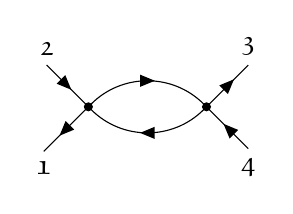
\begin{tikzpicture}[baseline=(current bounding box.center)]
    \begin{feynman}[small]
        % ph
        \vertex (i1);
        \vertex [dot, above right=0.75cm of i1] (i_left) {};
        \vertex [above left=0.75cm of i_left] (i4);
        \vertex [dot, right=1.5cm of i_left] (i_right) {};
        \vertex [below right=0.75cm of i_right] (i2);
        \vertex [above right=0.75cm of i_right] (i3);
        
        \vertex [below=0em of i1] {$\mathfrak 1$};
        \vertex [above=0em of i4] {$\mathfrak 2$};
        \vertex [above=0em of i3] {$\mathfrak 3$};
        \vertex [below=0em of i2] {$\mathfrak 4$};
        
        \diagram*{
            (i_left) -- [fermion] (i1),
            (i4) -- [fermion] (i_left),
            (i_right) -- [fermion] (i3),
            (i2) -- [fermion] (i_right),
            (i_left) -- [fermion, bend left=45] (i_right),
            (i_right) -- [fermion, bend left=45] (i_left),
        };
    \end{feynman}
\end{tikzpicture}
\begin{tikzpicture}[baseline=(current bounding box.center)]
    \begin{feynman}
        \vertex {$+$};
    \end{feynman}
\end{tikzpicture}
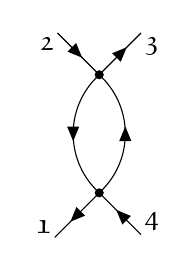
\begin{tikzpicture}[baseline=(current bounding box.center)]
    \begin{feynman}[small]
        % ph transversal
        \vertex (i1);
        \vertex [dot, above right=0.75cm of i1] (i_below) {};
        \vertex [below right=0.75cm of i_below] (i4);
        \vertex [dot, above=1.5cm of i_below] (i_above) {};
        \vertex [above left=0.75cm of i_above] (i2);
        \vertex [above right=0.75cm of i_above] (i3);
        
        \vertex [above left=-0.3em of i1] {$\mathfrak 1$};
        \vertex [above right=-0.3em of i4] {$\mathfrak 4$};
        \vertex [below right=-0.3em of i3] {$\mathfrak 3$};
        \vertex [below left=-0.3em of i2] {$\mathfrak 2$};
        
        \diagram*{
            (i_below) -- [fermion] (i1),
            (i4) -- [fermion] (i_below),
            (i_above) -- [fermion] (i3),
            (i2) -- [fermion] (i_above),
            (i_above) -- [fermion, bend right=45] (i_below),
            (i_below) -- [fermion, bend right=45] (i_above),
        };
    \end{feynman}
\end{tikzpicture}
\begin{tikzpicture}[baseline=(current bounding box.center)]
    \begin{feynman}
        \vertex {$+$};
    \end{feynman}
\end{tikzpicture}
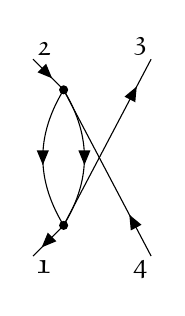
\begin{tikzpicture}[baseline=(current bounding box.center)]
    \begin{feynman}[small]
        % pp
        \vertex (i1);
        \vertex [right=1.5cm of i1] (i2);
        \vertex [above=2.5cm of i2] (i3);
        \vertex [left=1.5cm of i3] (i4);
        \vertex [dot, above right=0.5cm of i1] (i1_p) {};
        \vertex [dot, below right=0.5cm of i4] (i4_p) {};
        
        \vertex [below right=-0.3em of i1] {$\mathfrak 1$};
        \vertex [above right=-0.3em of i4] {$\mathfrak 2$};
        \vertex [above left=-0.3em of i3] {$\mathfrak 3$};
        \vertex [below left=-0.3em of i2] {$\mathfrak 4$};
        
        \diagram*{
            (i1_p) -- [fermion] (i1),
            (i1_p) -- [plain, with arrow=1.85cm] (i3),
            (i4) -- [fermion] (i4_p),
            (i2) -- [plain, with arrow=0.5cm] (i4_p),
            (i4_p) -- [fermion, bend left=30] (i1_p),
            (i4_p) -- [fermion, bend right=30] (i1_p),
        };
    \end{feynman}
\end{tikzpicture}

\end{document}